% !TeX root = ../economia.tex
\chapter{Decisioni di breve periodo}
Si tratta di decisioni che presentano \emph{effetti limitati nel tempo} e con \emph{risorse strutturali
fissate}.

\begin{itemize}
	\item Non mutano la struttura organizzativa e produttiva dell’impresa in
	modo sostanziale
	\item Non influenzano la strategia dell’impresa
	\item Hanno impatto economico-finanziario “limitato” rispetto investimenti di LP
	\item Gli investimenti in capitale fisico sono facilmente smobilizzabili nel lungo
	periodo
	\item Sono anche definite decisioni tattiche per contrapporle alle decisioni
	strategiche
\end{itemize}

\section{Costi fissi}

\begin{figure}[h]
	\centering
	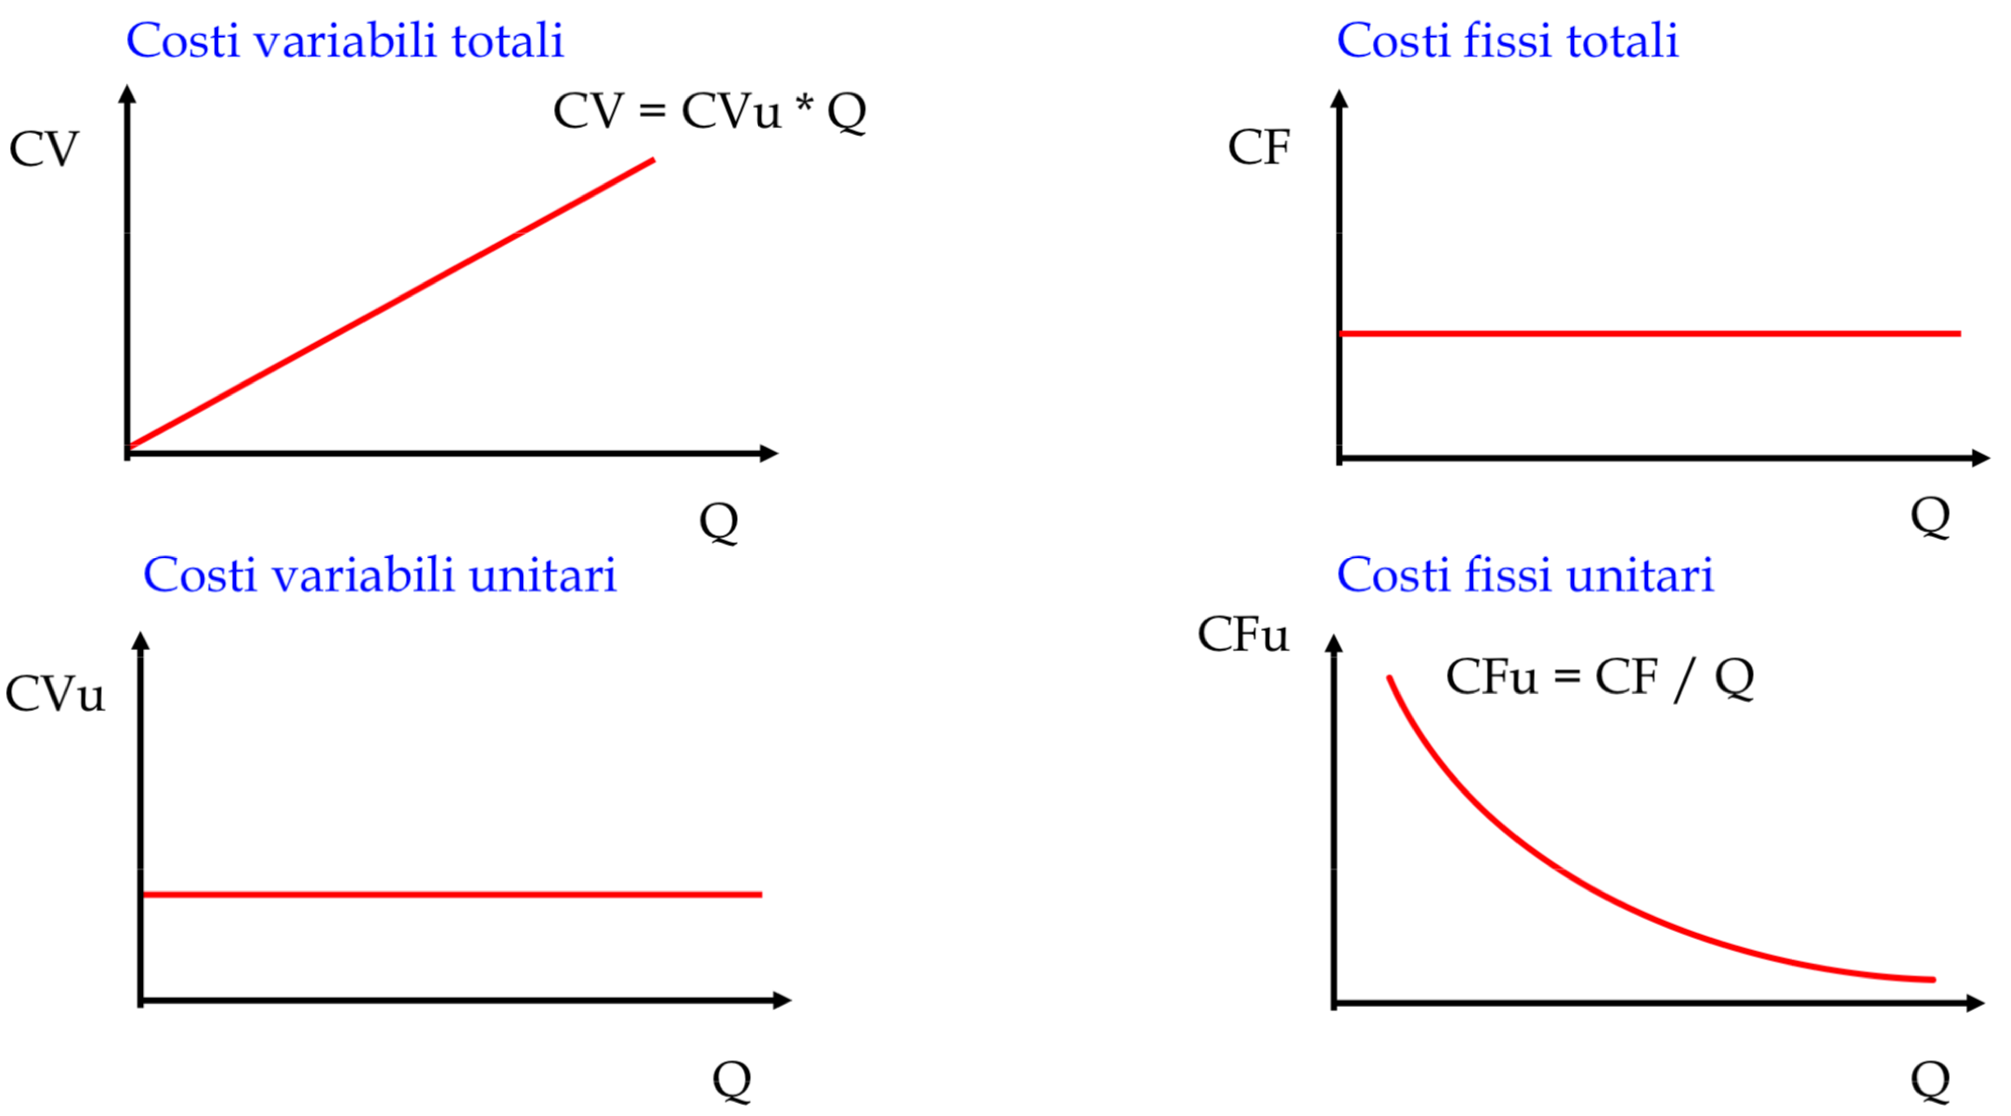
\includegraphics[width=0.5\linewidth]{images/costi}
	\caption{Costi fissi e costi variabili}
	\label{fig:costi}
\end{figure}

\paragraph{Costi totali}
\[
CT = CF + CV_u \times Q
\]
\paragraph{Margine di contribuzione unitario}
differenza tra prezzo di vendita e costo
variabile unitario.
\[
mc = p - CV_u
\]

\paragraph{Margine di contribuzione totale}
\[
MC = mc * Q \quad \textit{dove $Q$ \`e la quantit\`a prodotta}
\]
\paragraph{Margine di contribuzione medio}
Si definisce nel caso di impresa multi-prodotto
ponderando il margine di contribuzione del prodotto $j$-esimo per il rapporto $x_j$ tra il
volume di produzione del prodotto $j$-esimo e la produzione totale dell’azienda.
\[
x_j = Q_j / Q_{tot}
\]

\section{Analisi di break-even}
\subsection{Ipotesi semplificatrici}

\subsubsection{Ipotesi sui costi}
\begin{itemize}
	\item Non si considerano le economie di scala (aumento di costi meno che
proporzionale rispetto alla quantità)
	Possibili fonti di economie di scala sono: apprendimento, migliore
sfruttamento degli impianti
	\item Rendimenti (di scala) costanti
\end{itemize}

\subsubsection{Ipotesi sui ricavi}
\begin{itemize}
	\item I ricavi sono realizzati immediatamente (non sorgono crediti)
	\item Non vi sono scorte invendute
\end{itemize}

\subsubsection{Ipotesi sul prezzo}
\begin{itemize}
	\item Costante rispetto al volume di vendita
\end{itemize}

\subsection{Definizione}

L'analisi di break-even \`e una valutazione relativa a quanto è necessario produrre per:
\begin{itemize}
	\item Coprire i costi
	\item Ottenere un certo profitto
\end{itemize}

\subsection{Calcolo del punto di break-even}
$Q_{BE}$ \`e la quantit\`a di break-even.

Il MON \`e definito come:
\[
MON = RT - CT = p * Q - CV_u * Q - CF = p - CV_u * Q - CF = 0\\
Q_{BE} = \frac{CF}{p - CV_u} = \frac{CF}{mc}
\]

\subsubsection{Caso 1} determinazione del minimo volume operativo che consente il
pareggio tra ricavi e costi totali:
\[
Q_{BE} : \textit{\gls{MON}(EBIT)} = \textit{Ricavi}_{TOT} - \textit{Costi}_{TOT} = 0
\]

sotto le ipotesi semplificatrici, la quantità di break-even è:
\[
Q_{BE} = \frac{CF}{mc}
\]


Per le imprese multi-prodotto, supponendo che il mix produttivo sia definito da
percentuali prefissate $x_j$ di $N$ prodotti, la quantità di break-even del $j$-esimo
prodotto $Q_{BE_j}$ è:
\[
Q_{BE_j} = \frac{CF}{mc_\textit{medio}} x_j \\ mc_\textit{medio} = \sum^N_{j=1} mc_j \times x_j
\]

\subsubsection{Caso 2} determinazione del minimo volume operativo che permette
l'ottenimento di certi livelli di redditività:
\[
Q_{BE} : \textit{\gls{MON}(EBIT)} = \textit{Ricavi}_{tot} - \textit{Costi}_{tot} = \textit{Redditività auspicata}
\]

sotto le ipotesi semplificatrici, la quantità di break-even è:
\[
Q_{BE} = \frac{CF + \gls{MON}_\textit{target}}{mc}
\]

\subsection{Margine contribuzione percentuale}
Il punto di pareggio può anche essere espresso in termini percentuali sui ricavi
totali (RT). Moltiplicando entrambi i membri dell’equazione di break-even per il prezzo, si
ottiene:
\[
RT_{BE} = \frac{CF}{\frac{mc}{p}} = \frac{CF}{mc_\%}
\]

\subsection{Margine di sicurezza}
Il margine di sicurezza indica di quanto il volume di produzione attuale eccede il
volume di pareggio. Quindi il margine di sicurezza serve a rispondere alla seguente domanda: di
quanto possono ridursi i ricavi programmati prima di raggiungere il punto di
pareggio?

\paragraph{Esempio} se il volume attuale è pari a 200 unità ed il punto di pareggio è di
160 unità, il margine di sicurezza è pari a 40 unità, vale a dire al 20\% (40/200)
del volume attuale:
\begin{itemize}
	\item Il volume delle vendite può quindi diminuire del 20\% prima che si vada
	incontro ad una perdita
	\item È più significativo esprimere il margine di sicurezza in \% piuttosto che in
	valore assoluto (ms\% = 20\%)
\end{itemize}

\subsection{Pro e contro dei costi fissi}
\begin{multicols}{2}
	\begin{center}
		\textbf{Alta incidenza costi fissi}
	\end{center}
	\proandcons{Redditi alti in periodi di fatturato elevato}{Gravi crisi economiche in momenti di
		congiuntura sfavorevole e contrazione
		delle vendite}
	\vfill\null\columnbreak
	\begin{center}
		\textbf{Bassa incidenza costi fissi}
	\end{center}
	\proandcons{Risultati più stabili (meno variabili)}{Aumento inferiore del reddito quando i
		ricavi sono alti rispetto alle imprese con alta
		incidenza CF}
\end{multicols}

\section{Scelta di mix produttivo}
\begin{enumerate}
	\item Si calcola il margine di contribuzione di ciascun prodotto
	\item Si prendono in esame i vincoli:
	\begin{itemize}
		\item \emph{In assenza di vincoli:} si produce il prodotto con \textbf{margine di contribuzione
		maggiore}
		\item \emph{In presenza di vincoli di consumo di risorse:} \textbf{si massimizza il margine di
		contribuzione per risorsa scarsa}
		\item \emph{In presenza di vincoli di politiche aziendale:} si soddisfano gli eventuali
		vincoli di minimo di produzione e \textbf{si massimizza il margine di
		contribuzione} (o il margine di contribuzione per risorsa scarsa)
		\item \emph{In presenza di vincoli di mercato:} \textbf{si massimizza il margine di
		contribuzione} (o il margine di contribuzione per risorsa scarsa) senza
		superare i vincoli di massimo di produzione
	\end{itemize}

\end{enumerate}

\section{Scelte di make or buy}
Si tratta di decisioni inerenti la scelta tra:
\begin{itemize}
	\item Produrre un determinato prodotto (o componente/MP) all’interno
	dell’impresa (\emph{make})
	\item Acquistarlo sul mercato (\emph{buy})
\end{itemize}

Gli step della scelta sono:
\begin{enumerate}
	\item Si identificano le alternative di Make e Buy
	\item Si adotta una delle due alternative come caso base
	\item Si calcolano i costi e i ricavi differenziali al caso base
	\item Si preferisce l’alternativa che crea il maggior valore economico
\end{enumerate}

\subsection{Considerazioni}
Nelle scelte di make or buy può essere necessario tenere conto di \gls{costopport}.

Possono esistere anche scelte di \emph{make or buy} di lungo periodo, per esempio, se un’impresa deve scegliere se acquisire uno dei propri fornitori: i criteri decisionali adottati in questo caso sono più complessi e si ricorre alla valutazione
degli investimenti.

Le scelte di make or buy hanno degli evidenti limiti:
\begin{itemize}
	\item Prescindono da considerazioni di tipo qualitativo:
	\begin{itemize}
		\item Qualità del lavoro del fornitore
		\item Affidabilità del fornitore in termini di puntualità delle consegne
		\item Livello di riservatezza delle conoscenze necessarie a produrre un
		componente/prodotto
	\end{itemize}
	\item Non tengono conto dei costi di transazione (costi di organizzazione e gestione
	degli scambi)
	\item Non considerano l’opzione di collaborazione
\end{itemize}
